%pme2352
\section{Ex 1}

% \begin{figure}[h]
% \begin{center}
% \includegraphics[scale=0.48]{./fig/0.png}
% \caption{\label{fig:0} DCL} 
% \end{center}
% \end{figure}

\myfig{figPME2352-20111019-00}{DCL}

\paragraph*{Exemplo}

\[\mu _{r}R*\frac{\dot{x}}{|\dot{x}|}\footnote{ajuste de sinal}\]
\paragraph*{TMB}
\[m\ddot{x}=T-kx\]

\paragraph*{$TMA)_{CENTRO}$}
\[\frac{m R^{2}}{2}\ddot{\theta}=-T*R-\mu _{r}R\frac{\dot{x}}{|\dot{x}|}(mg)\footnote{Normal}\]

\[\theta R = x\]
\[\dot{\theta}R = \dot{x}\]
\[\ddot{\theta}R=\ddot{x}\]


\[m\ddot{x}=T-kx\]
\[\frac{m}{2}\ddot{x}=-T-\mu _{rol}\frac{\dot{x}}{|\dot{x}|}mg\]
\[\frac{3m}{2}\ddot{x}=-kx-\mu _{rol}\frac{\dot{x}}{|\dot{x}|}mg\]
\[\frac{3m}{2}\ddot{x}+kx+\mu _{rol}\frac{\dot{x}}{|\dot{x}|}mg=0\]

% \begin{figure}[h]
% \begin{center}
% 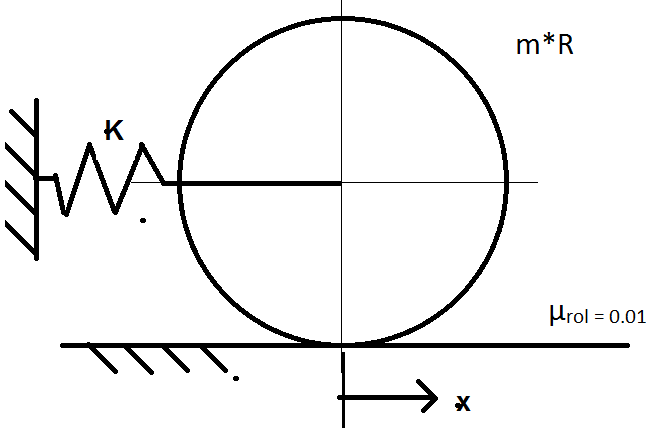
\includegraphics[scale=0.48]{./fig/0-1.png}
% \caption{\label{fig:01} Exemplo} 
% \end{center}
% \end{figure}

\myfig[scale=.48]{figPME2352-20111019-01}{}

\[m_{eq}\ddot{x}+c_{eq}\dot{x} +k_{eq}x=0\]

% \begin{figure}[h]
% \begin{center}
% 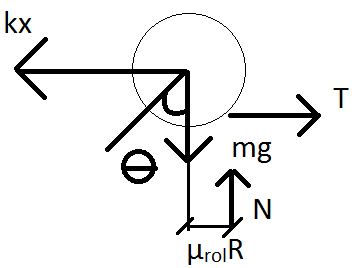
\includegraphics[scale=0.78]{./fig/0-2.png}
% \caption{\label{fig:02} DCL exemplo} 
% \end{center}
% \end{figure}

\myfig{figPME2352-20111019-02}{}

Para $\dot{x}>$  0
\[\frac{3m}{2}\ddot{x}+kx+\mu _{rol}mg=0\]

Para $\dot{x}<$  0
\[\frac{3m}{2}\ddot{x}+kx-\mu _{rol}mg=0\]

\begin{itemize}
  \item $\dot{x}(0)=0$
\end{itemize}

Para t$>$0, para t $<$ T
\[(2a+b)\ddot{x}+2gx=0(t)\]

% \begin{figure}[h]
% \begin{center}
% \includegraphics[scale=0.25]{./fig/0-3.png}
% \caption{\label{fig:1}2 ex1} 
% \end{center}
% \end{figure}

\myfig{figPME2352-20111019-03}{}

\section{Ex 2}

% \begin{figure}[h]
% \begin{center}
% 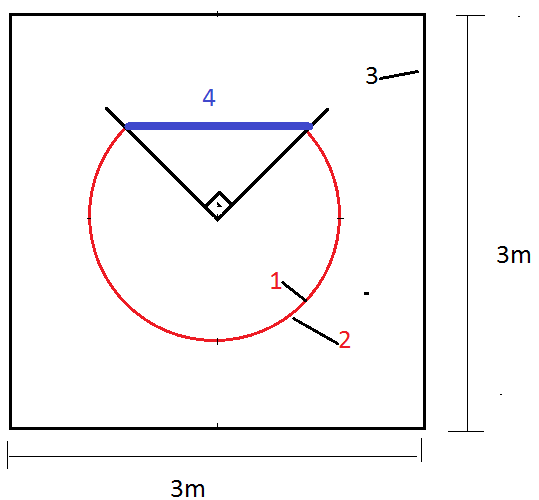
\includegraphics[scale=0.48]{./fig/1.png}
% \caption{\label{fig:1}1 Ex 2} 
% \end{center}
% \end{figure}

\myfig{figPME2352-20111019-04}{}

% \begin{figure}[h]
% \begin{center}
% 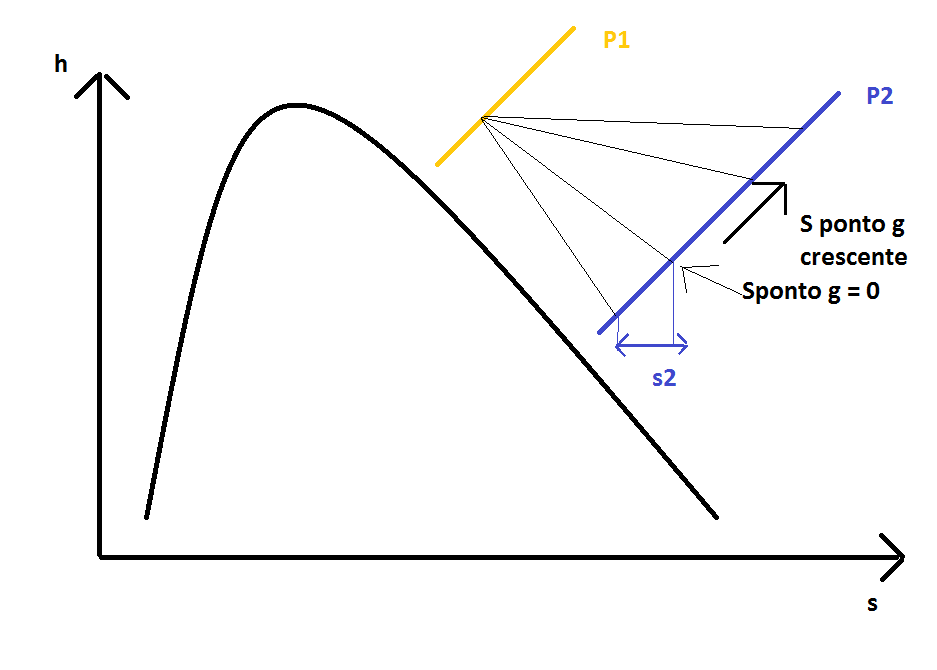
\includegraphics[scale=0.16]{./fig/2.png}
% \caption{\label{fig:1}2 Ex 2} 
% \end{center}
% \end{figure}

\myfig{figPME2352-20111019-05}{}

\[2(\rho A a)\ddot{x}+\rho A b(\ddot{x}+\dot{v}(t))=-2x\rho gA\]

\[(2a+b)\ddot{x}+2gx=-b\dot{v}(t)\]
\[m_{eq}\ddot{x}+k_{eq}x=\psi(t)\]

\[\omega = \sqrt{\frac{2g}{2a+b}}\]
Para 0$<$t$<$T
\[(2a+b)\ddot{x}+2gx=b\frac{V_{0}}{T}\]
Condiçeos iniciais:
\begin{itemize}
\item x(0)=0

\item $\dot{x}(0)=0$
\end{itemize}
Para t$<$0, para t $>$ T
\[(2a+b)\ddot{x}+2gx=0(t)\]

% \begin{figure}[h]
% \begin{center}
% 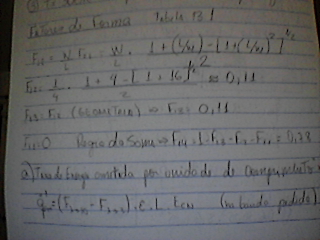
\includegraphics[scale=0.28]{./fig/3.png}
% \caption{\label{fig:1} F de $\tau$} 
% \end{center}
% \end{figure}

\myfig{figPME2352-20111019-06}{}

\[x(t)=\frac{1}{m\omega} \int _{0}^{t} {F(\tau)\sin(\omega(t-\tau))d\tau}\]

\[x_{h}(t)=A\sin(\omega t)+B\cos(\omega t)\]
\[x_{p}(t)=\frac{bV_{0}}{2gT}\]

\[x(t)=A\sin(\omega t)+B\cos(\omega t)+\frac{bV_{0}}{2gT}\]

\[\dot{x}(t)=A\omega \cos(\omega t)-B\sin(\omega t)\]
Condições Iniciais:

\[x(0)=0=B+\frac{bV_{0}}{2gT}\]
\[\dot{x}(0)=0=A\omega\]
Portanto
\[B=-\frac{-bV_{0}}{2gT}\]
\[A=0\]

\[x(t)=\frac{bV_{0}}{2gT}(1-\cos(\omega t))\]
\[\dot{x} (t)=\frac{bV_{0}}{2gT}\omega \sin(\omega t)\]

% \begin{figure}[h]
% \begin{center}
% 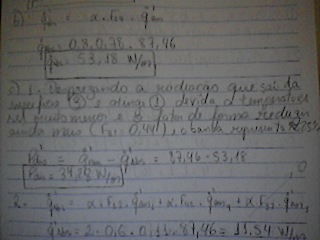
\includegraphics[scale=0.28]{./fig/5.png}
% \caption{\label{fig:5}Para 0$<$  t $<$T;$\omega t = 2\pi$} 
% \end{center}
% \end{figure}

\myfig{figPME2352-20111019-07}{}

Para t=T:
\[x(T)=\frac{bV_{0}}{2gT}(1-\cos(\omega t))\]
\[\dot{x}(T)=\frac{bV_{0}}{2gT}\omega \sin(\omega t)\]
Para t$>$ T
\[(2a+b)\ddot{x}+2gx=0\]
\[A'\sin(\omega t)+B'\cos(\omega t)\]
\[A' \omega\cos(\omega t)-B' \omega\sin(\omega t)\]

CI do trecho:
\[x(T)=\frac{bV_{0}}{2gT}(1-\cos(\omega t))=A'\sin(\omega t)+B'\cos(\omega t)\]
\[\dot{x}(T)=\frac{bV_{0}}{2gT}(\omega \sin(\omega t))=A' \omega\cos(\omega t)-B'\sin(\omega t)\]